\documentclass[12pt]{article}
\usepackage{amsmath}
%\usepackage{fullpage}
\usepackage[top=1in, bottom=1in, left=0.8in, right=1in]{geometry}
\usepackage{multicol}
\usepackage{wrapfig}
\usepackage{graphicx}
\usepackage{float}
\usepackage{listings}
\usepackage{enumerate}
\lstset{language=Java,
	basicstyle={\small\ttfamily},
	columns=flexible,
	belowskip=0mm}

\setlength{\columnsep}{0.1pc}

\title{ME573 Homework Set \# 11}
\author{Alexander Swenson -- \texttt{aaswenson@wisc.edu}}
\date{\today}
\begin{document}
	
	\maketitle
	
	\vspace{-0.3in}
	\noindent
	\rule{\linewidth}{0.4pt}
	
	\noindent
	

\section{Problem 1}
	See attached screenshots from Mathematica for problem 1. The screenshots support the exact solutions validity as a solution to the underlying PDE.

\section{Problem 2}
	
\noindent Displayed below is the matrix form of the first two steps in the algorithm.
\subsection{(1-a)}	
\[
\begin{bmatrix} 
4(1+\alpha_x) & (\frac{u_{2,j}^n\Delta t}{\Delta x} - 2\alpha)   &			   &\\
-(\frac{u_{3,j}^n\Delta t}{\Delta x} + 2\alpha) & 4(1+\alpha_x) & (\frac{u_{3,j}^n\Delta t}{\Delta x} - 2\alpha)  &\\
& \ddots &			   &\\
&	 	  & \ddots & (\frac{u_{N-2,j}^n\Delta t}{\Delta x} - 2\alpha)  \\
&		  & -(\frac{u_{3,j}^n\Delta t}{\Delta x} + 2\alpha) & 4(1+\alpha_x)  \\ 
\end{bmatrix}
\begin{bmatrix} 
f_{2,j}^{*}\\
f_{3,j}^{*}\\
\vdots\\
f_{Nx-2,j}^{*}\\
f_{Nx-1,j}^{*}\\ 
\end{bmatrix} = 
\begin{bmatrix} 
b_{2,j}^n\\
b_{3,j}^n\\
\vdots\\
b_{N-2,j}^n\\
b_{N,j}^n\\ 
\end{bmatrix}
\]

Where:

\begin{equation}
	b_{i,j}^n = (\frac{u_{i,j}^n\Delta t}{\Delta x} + 2 \alpha_x)u_{i-1,j}^n + 4(1-\alpha_x)u_{i,j}^n + (2 \alpha_x - \frac{u_{i,j}^n\Delta t}{\Delta x})u_{i+1,j}^n
\end{equation}

\begin{equation}
	b_{2,j} = (\frac{u_{2,j}^n\Delta t}{\Delta x} + 2 \alpha_x)u_{1,j}^*
\end{equation}

\begin{equation}
b_{N-1,j} = ( 2 \alpha_x - \frac{u_{N-1,j}^n\Delta t}{\Delta x} +)u_{N,j}^*
\end{equation}
\subsection{(1-b)}	
\[
\begin{bmatrix} 
4(1+\alpha_y) & (\frac{v_{2,j}^n\Delta t}{\Delta x} - 2\alpha)   &			   &\\
-(\frac{v_{3,j}^n\Delta t}{\Delta x} + 2\alpha) & 4(1+\alpha_y) & (\frac{v_{3,j}^n\Delta t}{\Delta x} - 2\alpha)  &\\
& \ddots &			   &\\
&	 	  & \ddots & (\frac{v_{N-2,j}^n\Delta t}{\Delta x} - 2\alpha)  \\
&		  & -(\frac{v_{3,j}^n\Delta t}{\Delta x} + 2\alpha) & 4(1+\alpha_y)  \\ 
\end{bmatrix}
\begin{bmatrix} 
f_{2,j}^{*}\\
f_{3,j}^{*}\\
\vdots\\
f_{Nx-2,j}^{*}\\
f_{Nx-1,j}^{*}\\ 
\end{bmatrix} = 
\begin{bmatrix} 
b_{2,j}^n\\
b_{3,j}^n\\
\vdots\\
b_{N-2,j}^n\\
b_{N,j}^n\\ 
\end{bmatrix}
\]

Where:

\begin{equation}
b_{i,j}^n = (\frac{v_{i,j}^n\Delta t}{\Delta x} + 2 \alpha_y)v_{i-1,j}^n + 4(1-\alpha_y)v_{i,j}^n + (2 \alpha_y - \frac{v_{i,j}^n\Delta t}{\Delta x})v_{i+1,j}^n
\end{equation}

\begin{equation}
b_{2,j} = (\frac{v_{2,j}^n\Delta t}{\Delta x} + 2 \alpha_y)v_{1,j}^*
\end{equation}

\begin{equation}
b_{N-1,j} = ( 2 \alpha_y - \frac{v_{N-1,j}^n\Delta t}{\Delta x} +)v_{N,j}^*
\end{equation}

\subsection{Time Domain}
Since this is a steady state solution, I needed to ensure my approximation had reached steady state. If the solution was still transient, it would not match the exact solution. I controlled this with the number of time steps taken and the length of the time step used. I used trial and error to determine the sufficient number of time steps and step length to model the underlying PDE. 

For FTCS I used dt = 0.001 and tf=15. For CN I used dt=0.1 and tf=15. Due to the extra iterations required for FTCS, it took much more time to run. Using the tic, toc, method in Matlab (and including the overhead to set up the problem for both CN and FTCS), the Crank-Nicolson and FTCS methods took, 10.44 and 5.8 seconds respectively.

\subsection{Error Plots}

Below are the error plots for the steady state FD solutions compared to the exact solution. I should note that the error of the x-component (u) of the solution is too high for FTCS. I have not been able to determine the source of this error. I was encouraged by the error performance of the y-component for FTCS and both component results using CN.

	\begin{figure}[!htb]
		\centering
		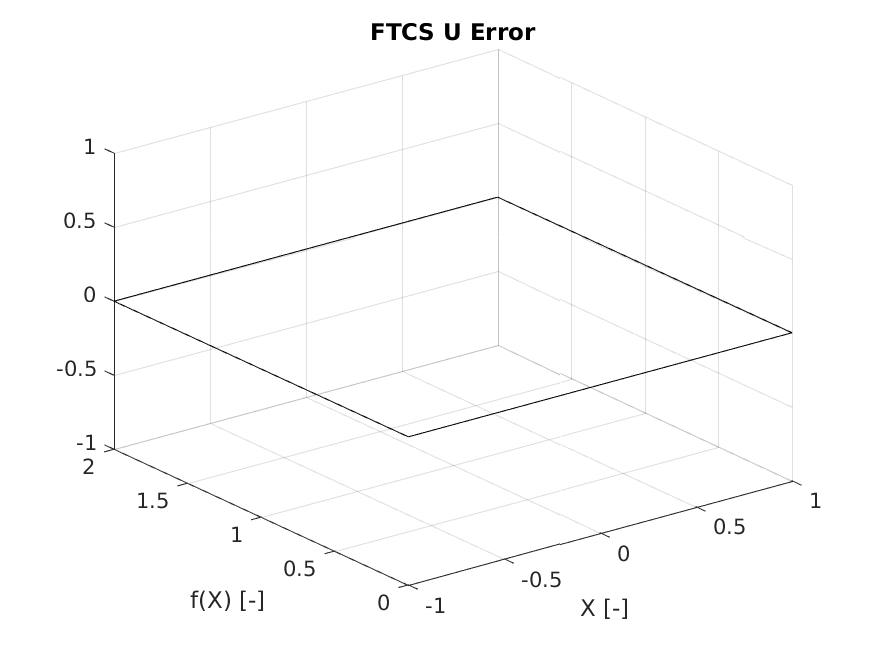
\includegraphics[scale=0.75]{ftcsu.png}
	\end{figure}
	
	\begin{figure}[!htb]
		\centering
		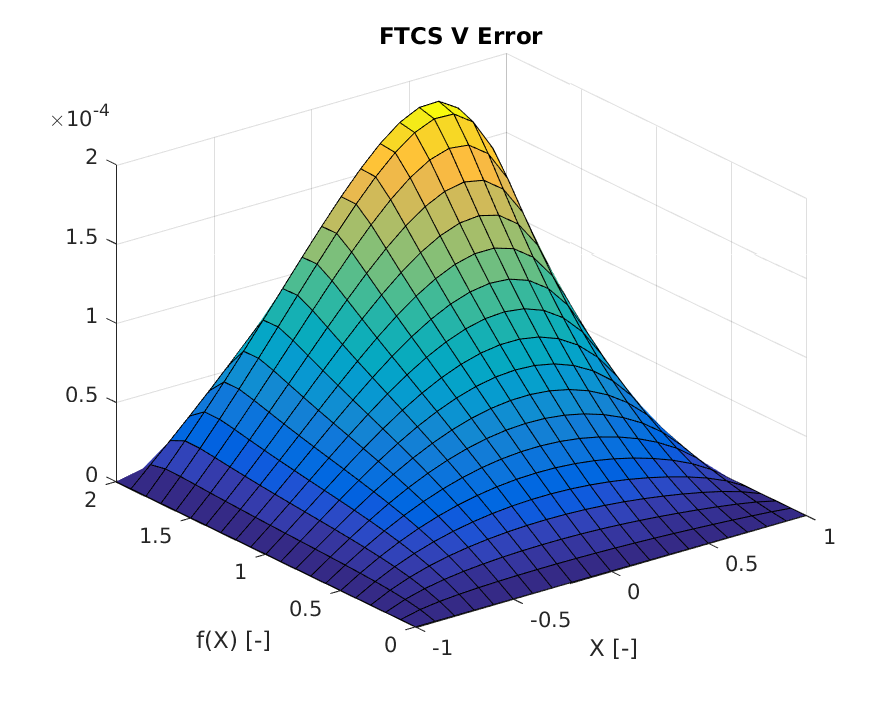
\includegraphics[scale=0.75]{ftcsv.png}
	\end{figure}
	
	\begin{figure}[!htb]
		\centering
		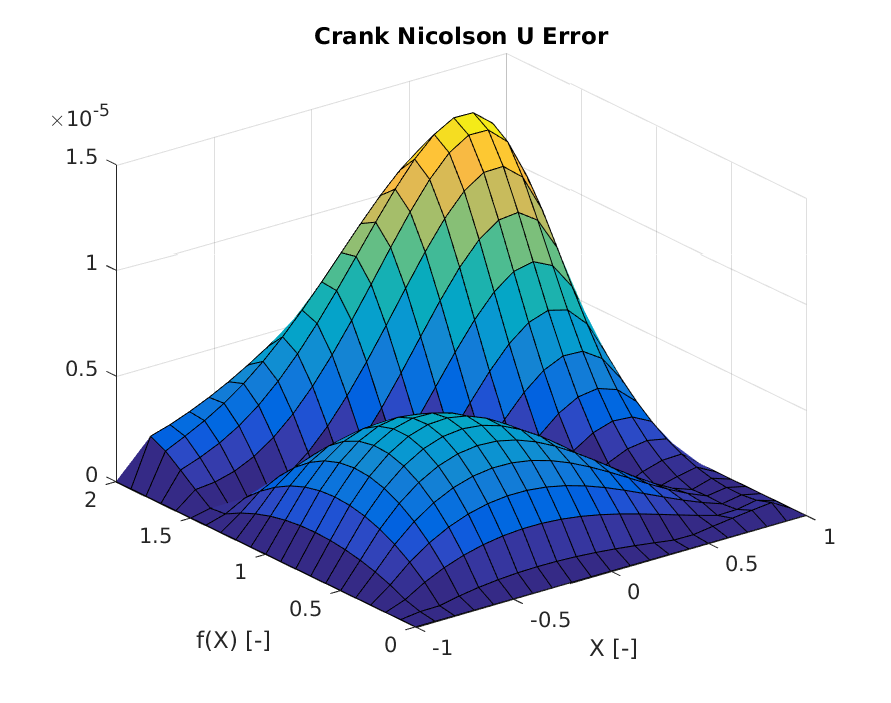
\includegraphics[scale=0.75]{CNu.png}
	\end{figure}
	
	\begin{figure}[!htb]
		\centering
		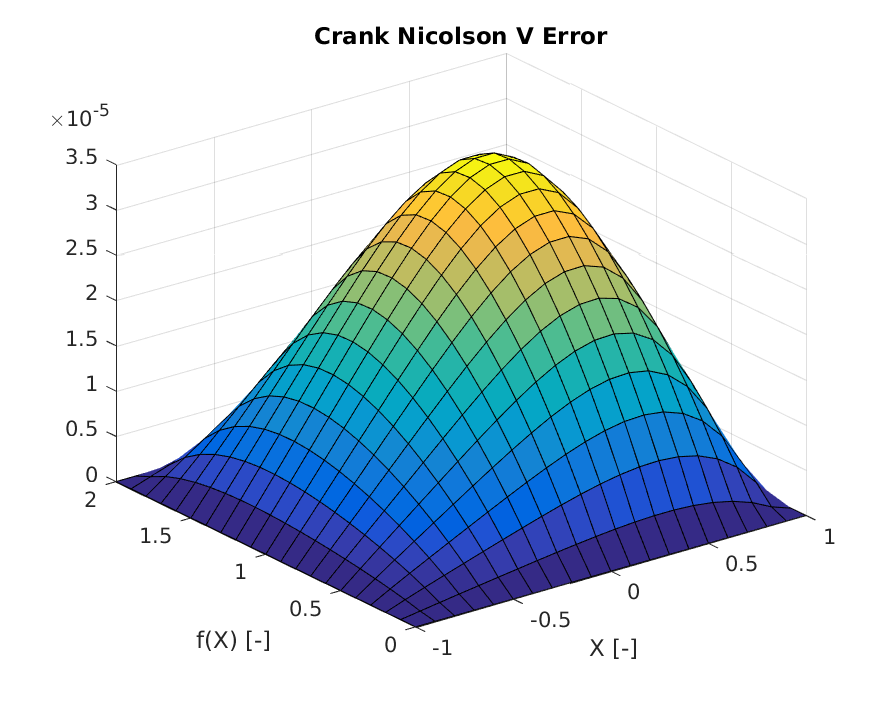
\includegraphics[scale=0.75]{CNv.png}
	\end{figure}

%%%%%%%%%%%%%%%%%%%%%%%%%%%%%%%%%%%%%%%%%%%%%%%%%%%%%%%%%%%%%%%%%%%%%%%%%%%%%%%%

		
	
	
	
	
\end{document}
